\documentclass{article}
\usepackage[a4paper, margin=2cm]{geometry}

\usepackage{amsmath}
\usepackage{amssymb}
\usepackage{mathtools}
\usepackage{amstext}
\usepackage{amsthm}
\usepackage{mathrsfs}
\usepackage{bm}
\usepackage{fancyhdr}
\usepackage{centernot}
\usepackage[ruled,vlined]{algorithm2e}

\usepackage{hyperref}

\usepackage{graphicx}
\usepackage{float}
\usepackage{caption}
\usepackage{subcaption}

\usepackage{booktabs, multirow}

\usepackage{tikz}
\usetikzlibrary{patterns}
\usepackage{pgfplots}
\pgfplotsset{compat=1.15}
\usetikzlibrary{arrows}

% To work with inkfigures
\usepackage{import}
\usepackage{pdfpages}
\usepackage{transparent}
\usepackage{xcolor}

\newcommand{\incfig}[2][1]{%
    \def\svgwidth{#1\columnwidth}
    \import{./figures/}{#2.pdf_tex}
}

\pdfsuppresswarningpagegroup=1

%\graphicspath{{figures/}}

\pagestyle{fancy}
\rhead{Alexandre Adam}
\lhead{Probabilistic Graphical Models \\ Simon Lacoste-Julien}
\chead{Homework 3}
\rfoot{\today}
\cfoot{\thepage}

\newcommand{\angstrom}{\textup{\AA}}
\numberwithin{equation}{section}
\renewcommand\thesubsection{\alph{subsection})}
\renewcommand\thesubsubsection{\Roman{subsubsection}}
\newcommand{\s}{\hspace{0.1cm}}

\newcommand{\indep}{\s \rotatebox[origin=c]{90}{$\models$}\s }

%\tikzset{%
        %observed/.style={pattern=north west lines, pattern color=gray}
        %active_path/.style={->|, dashed, thick, blue}
%}
\newtheorem*{theorem}{Theorem}

\newtheoremstyle{named}{}{}{\itshape}{}{\bfseries}{.}{.5em}{\thmnote{#3's }#1}
\theoremstyle{named}
\newtheorem*{namedtheorem}{Theorem}
\tikzset{>=latex}

\begin{document}
\section{DGM}
We consider $G$, a DAG:
\begin{figure}[H]
        \centering
        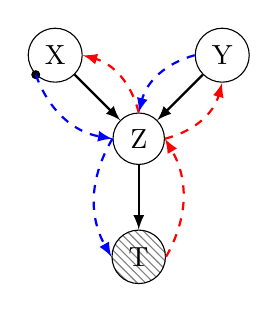
\begin{tikzpicture}
                % cbr = child below right, pbl = parent below left (snippets)
                \tikzstyle{every node}=[circle, draw=black, node distance=1.5cm]
                \tikzstyle{every edge}=[black, ->, thick, draw]
                \node (Z) at (0, 0) {Z};
                \node (Y) [above right of = Z] {Y};
                \draw (Y) edge (Z);
                \node (X) [above left of = Z] {X};
                \draw (X) edge (Z);
                \node[pattern=north west lines, pattern color=gray] (T) [below of = Z] {T};
                \draw (Z) edge (T);
                \node[circle, fill=black, inner sep=1pt] at (X.south west) {}; 

                % bayes ball

                \draw[->, blue, dashed, thick, bend right] (X.south west) to 
                        (Z.west);


                \draw[->, blue, dashed, thick, bend right] (Z.west) to 
                        (T.west);

                \draw[->, red, dashed, thick, bend right] (T.east) to 
                        (Z.east);

                \draw[->, red, dashed, thick, bend right] (Z.east) to 
                        (Y.south);

                
                \draw[->, blue, dashed, thick, bend right] (Y.west) to 
                        (Z.north);

                \draw[->, red, dashed, thick, bend right] (Z.north) to 
                        (X.east);
                
        \end{tikzpicture}
        \caption{Graph $G$, where $T$ is observed. An active path (blue dashed line) can lead 
        from $X$ to $Y$ since this is an undirected path. The arrow is there to indicate the 
        motion of the Bayes Ball. The starting point of the algorithm is represented as a 
black dot.}
        \label{fig:DGM1}
\end{figure}
A distribution $p\in \mathcal{L}(G)$ satisfy the factorization 
\[
        p(x_V) = p(x)p(y)p(z \mid x, y) p(t \mid z)
\]
From figure \ref{fig:DGM1}, we understand the statement $X \indep Y \mid T$ should be false 
in general. The following example show a case where this is indeed false.

Consider $(X, Y, Z, T)$ to be a vector of binary variables. 
\begin{enumerate}
        \item $X$ and $Y$ are independent coin flips;
        \item $Z$ has some high probability to be $1$ if $X = Y$;
        \item $Z$ has some high probability to be zero otherwise;
        \item $T$ has some high probability to be $1$ when $Z = 1$;
        \item $T$ has some high probability to be $0$ when $Z = 0$.
\end{enumerate}
We are given that $T = 1$. Here, the conditional independence is clearly false 
since 
\[
        p(x=1 \mid t=1, y=1) > p(x=1 \mid t=1, y=0)
\]
Therefore, 
\[
        p(x \mid t, y) \not= p(x  \mid t)
\]



%To prove that $X \indep Y \mid T$, we use the Bayes Ball algorithm (see algorithm 
%\ref{alg:Bayes} in the appendix). We conclude that $\boxed{X \centernot\indep Y 
%\mid T}$ because there exists an undirected active path (blue dashed line in figure 
%\ref{fig:DGM1}) from $X$ to $Y$. This could also have been observed using the fact that
%the unobserved node $Z$ with two parents has a descendant that is 
%observed. 
%As can be seen in figure \ref{fig:DGM1}, there is no active path between $X$ and $Y$ even 
%though $T$ is observed. Therefore, $X$ and $Y$ are \textbf{d-separated} by $T$ and 
%the conditional independence 
%\[
        %X \indep Y \mid T
%\]
%holds for $p \s \in \s \mathcal{L}(G)$. $\qed$


%where $\pi_i$ is the set of all parents of node $i$ and $V$ is the set of vertex in the graph. 
%From this definition, $p$ is a distribution of $\mathcal{L}(G)$ if the 
%following conditional independence relation holds
%\[
        %p \s \in \mathcal{L}(G) \iff X_i \indep X_{nd(i)} \mid X_{\pi_i}\s \forall \s i
%\]
%Therefore, $p\in  \mathcal{L}(G)$ must satisfy 

\section{D-separation in DGM}
We consider the graph $G$:
\begin{figure}[H]
        \centering
        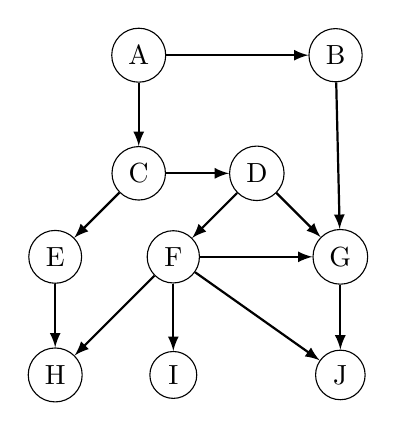
\begin{tikzpicture}
                % cbr = child below right, pbl = parent below left (snippets)
                \tikzset{>=latex}
                \tikzstyle{every node}=[circle, draw=black, node distance=1.5cm]
                \tikzstyle{every edge}=[black, ->, thick, draw]
                \node (A) at (0, 0) {A};
                \node (B) [right of = A, node distance=2.5cm] {B};
                \draw (A) edge (B);
                \node (C) [below of = A] {C};
                \draw (A) edge (C);
                \node (D) [right of = C] {D};
                \draw (C) edge (D);
               \node (E) [below left of = C] {E};
               \draw (C) edge (E);
               \node (H) [below of = E] {H};
               \draw (E) edge (H);
               \node (F) [below left of = D] {F};
               \draw (D) edge (F);
               \node (G) [below right of = D] {G};
               \draw (D) edge (G);
               \draw (F) edge (G);
               \node (I) [below of = F] {I};
               \draw (F) edge (I);
               \node (J) [below of = G] {J};
               \draw (G) edge (J);
               \draw (F) edge (H);
               \draw (F) edge (J);
               \draw (B) edge (G);
        \end{tikzpicture}
        \caption{Complete graph $G$.}
        \label{fig:G2}
\end{figure}

We are interested in the verification of several conditional independence relations. For each 
case, we will verify the relation using Bayes Ball algorithm (see algorithm \ref{alg:Bayes}). 
Here, we exploit the fact that unobserved node do not have the ability to bounce the ball 
when visited by a parent. Therefore, for each cases, we only consider a relevant sub-graph 
of $G$ built by plucking away all the unobserved nodes until an observed node is found or 
a node of interest is found.
\pagebreak
\renewcommand{\arraystretch}{2}
\begin{table}[H]
        \centering
        \begin{tabular}{ccc}
                Relevant sub-graph &  Conditional independence & True/False \\
                \hline
                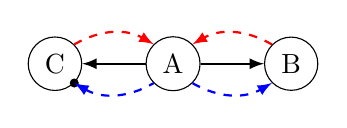
\begin{tikzpicture}[baseline=(current bounding box.center)]
                        % cbr = child below right, pbl = parent below left (snippets)
                        \tikzstyle{every node}=[circle, draw=black, node distance=1.5cm]
                        \tikzstyle{every edge}=[black, ->, thick, draw]
                        \node (C) at (0, 0) {C};
                        \node (A) [right of = C] {A};
                        \draw (A) edge (C);
                        \node (B) [right of = A] {B};
                        \node[circle, fill=black, inner sep=1pt] at (C.south east) {};
                        \draw (A) edge (B);
                        \draw[<-, blue, dashed, thick, bend right] (C.south east) to 
                                (A.south west);
                        \draw [->, blue, dashed, thick, bend right] (A.south east) to 
                                (B.south west);

                        \draw[->, red, dashed, thick, bend left] (C.north east) to 
                                (A.north west);


                        \draw[->, red, dashed, thick, bend right] (B.north west) to  
                                (A.north east);

                \end{tikzpicture}
                                  & $C \indep B \mid \emptyset$ & False \\
                \cmidrule{2-3}

                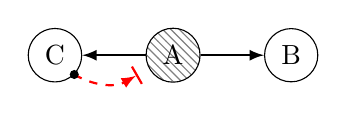
\begin{tikzpicture}[baseline=(current bounding box.center)]

                        % cbr = child below right, pbl = parent below left (snippets)
                        \tikzset{>=latex}
                        \tikzstyle{every node}=[circle, draw=black, node distance=1.5cm]
                        \tikzstyle{every edge}=[black, ->, thick, draw]
                        \node[pattern=north west lines, pattern color=gray] (A) at (0, 0) {A};
                        \node (C) [left of = A] {C};
                        \draw (A) edge (C);
                        \node (B) [right of = A] {B};
                        \draw (A) edge (B);
                        
                        \draw[->|, red, dashed, thick, bend right] (C.south east) to 
                                ([xshift=-0.2cm]A.south west);
                        \node[circle, fill=black, inner sep=1pt] at (C.south east) {};
     %                   \draw [->|, red, dashed, thick, bend left] (B.south west) to 
                                %([xshift=0.2cm]A.south east);
                \end{tikzpicture}
                                  & $C \indep B \mid A $ & True \\
                                  \cmidrule{2-3}
                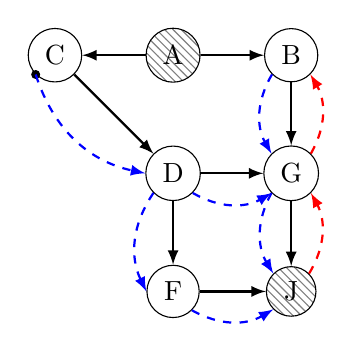
\begin{tikzpicture}[baseline=(current bounding box.center)]
                        % cbr = child below right, pbl = parent below left (snippets)
                        \tikzstyle{every node}=[circle, draw=black, node distance=1.5cm]
                        \tikzstyle{every edge}=[black, ->, thick, draw]
                        \node[pattern=north west lines, pattern color=gray] (A) at (0, 0) {A};
                        
                        \node (C) [left of = A] {C};
                        \node[circle, fill=black, inner sep=1pt] at (C.south west) {};
                        \draw (A) edge (C);
                        \node (B) [right of = A] {B};
                        \draw (A) edge (B);

                        \node (D) [below of = A] {D};
                        \draw (C) edge (D);
                        \node (G) [below of = B] {G};
                        \draw (B) edge (G);
                        \draw (D) edge (G);
                        \node (F) [below of = D] {F};
                        \draw (D) edge (F);
                        \node[pattern=north west lines, pattern color=gray] (J) [below of = G] {J};
                        \draw (G) edge (J);
                        \draw (F) edge (J);

                        
                        \draw [->, blue, dashed, thick, bend right] (C.south west) to 
                                (D.west);

                        \draw[->, blue, dashed, thick, bend right] (D.south west) to 
                                (F.west);

                        \draw[->, blue, dashed, thick, bend right] (D.south east) to 
                                (G.south west);

                        \draw[->, blue, dashed, thick, bend right] (F.south east) to 
                                (J.south west);

                        \draw[->, red, dashed, thick, bend right] (J.north east) to 
                                (G.south east);

                        \draw[->, blue, dashed, thick, bend right] (G.south west) to 
                                (J.north west);

                        \draw[->, red, dashed, thick, bend right] (G.north east) to 
                                (B.south east);


                        \draw[->, blue, dashed, thick, bend right] (B.south west) to 
                                (G.north west);
                        
                        
                \end{tikzpicture}
                                  & $C \indep B \mid A ,J$ & False \\ 
                                  \cmidrule{2-3}

                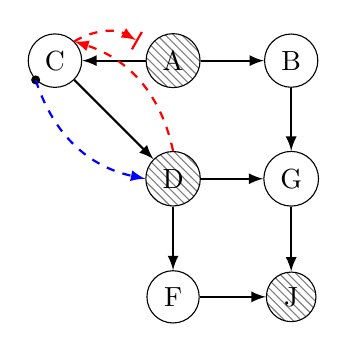
\begin{tikzpicture}[baseline=(current bounding box.center)]
                        % cbr = child below right, pbl = parent below left (snippets)
                        \tikzstyle{every node}=[circle, draw=black, node distance=1.5cm]
                        \tikzstyle{every edge}=[black, ->, thick, draw]
                        \node[pattern=north west lines, pattern color=gray] (A) at (0, 0) {A};
                          
                        \node (C) [left of = A] {C};
                        \draw (A) edge (C);
                        \node (B) [right of = A] {B};
                        \draw (A) edge (B);
                        
                        %\draw[->|, blue, dashed, thick, bend right] (C.south east) to 
                                %([xshift=-0.2cm]A.south west);
                        %\draw [->|, blue, dashed, thick, bend left] (B.south west) to 
                                %([xshift=0.2cm]A.south east);

                        \node[pattern=north west lines, pattern color=gray] (D) [below of = A] {D};
                        \draw (C) edge (D);
                        \node (G) [below of = B] {G};
                        \draw (B) edge (G);
                        \draw (D) edge (G);
                        \node (F) [below of = D] {F};
                        \draw (D) edge (F);
                        \node[pattern=north west lines, pattern color=gray] (J) [below of = G] {J};
                        \draw (G) edge (J);
                        \draw (F) edge (J);
                        \node[circle, fill=black, inner sep=1pt] at (C.south west) {};
                        
                        \draw [->, blue, dashed, thick, bend right] (C.south west) to 
                                (D.west);

                        \draw[->, red, dashed, thick, bend right] (D.north) to 
                                (C.north east);

                        \draw[->|, red, dashed, thick, bend left] (C.north east) to 
                                ([xshift=-0.2cm]A.north west);

                \end{tikzpicture}
                                  & $C \indep B \mid A,J,D$ & True \\
                                  \cmidrule{2-3}
                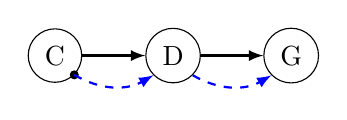
\begin{tikzpicture}[baseline=(current bounding box.center)]
                        % cbr = child below right, pbl = parent below left (snippets)
                        \tikzstyle{every node}=[circle, draw=black, node distance=1.5cm]
                        \tikzstyle{every edge}=[black, ->, thick, draw]
                        \node (C) at (0, 0) {C};
                        \node (D) [right of = C] {D};
                        \draw (C) edge (D);
                        \node (G) [right of = D] {G};
                        \draw (D) edge (G);
                        \node[circle, fill=black, inner sep=1pt] at (C.south east) {};

                        \draw[->, blue, dashed, thick, bend right] (C.south east) to 
                                (D.south west);

                        \draw[->, blue, dashed, thick, bend right] (D.south east) to 
                                (G.south west);

                        %\draw[->, red, dashed, bend right] (G.north west) to 
                                %(D.north east);

                        %\draw[->, red, dashed, bend right] (D.north west) to 
                                %(C.north east);
                        
                \end{tikzpicture}
                                  & $C \indep G \mid \emptyset$ & False \\
                                  \cmidrule{2-3}
                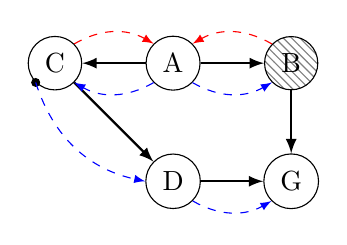
\begin{tikzpicture}[baseline=(current bounding box.center)]
                        % cbr = child below right, pbl = parent below left (snippets)
                        \tikzstyle{every node}=[circle, draw=black, node distance=1.5cm]
                        \tikzstyle{every edge}=[black, ->, thick, draw]
                        \node (A) at (0, 0) {A};
                        \node (C) [left of = A] {C};
                        \node[circle, fill=black, inner sep=1pt] at (C.south west) {};
                        \draw (A) edge (C);
                        \node[pattern=north west lines, pattern color=gray] (B) [right of = A] {B};
                        \draw (A) edge (B);
                        \node (D) [below of = A] {D};
                        \draw (C) edge (D);
                        \node (G) [below of = B] {G};
                        \draw (B) edge (G);
                        \draw (D) edge (G);

                        \draw[->, blue, dashed, bend right] (C.south west) to 
                                (D.west);

                        \draw[->, blue, dashed, bend right] (D.south east) to 
                                (G.south west);

                        \draw[->, red, dashed, bend left] (C.north east) to 
                                (A.north west);

                        \draw[->, blue, dashed, bend right] (A.south east) to 
                                (B.south west);

                        \draw[->, red, dashed, bend right] (B.north west) to 
                                (A.north east);


                        \draw[->, blue, dashed, bend left] (A.south west) to 
                                (C.south east);
                \end{tikzpicture}
                                  & $C \indep G \mid B$ & False \\
                          \cmidrule{2-3}
                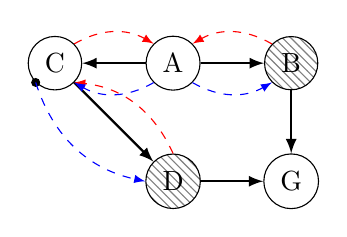
\begin{tikzpicture}[baseline=(current bounding box.center)]
                        % cbr = child below right, pbl = parent below left (snippets)
                        \tikzset{>=latex}
                        \tikzstyle{every node}=[circle, draw=black, node distance=1.5cm]
                        \tikzstyle{every edge}=[black, ->, thick, draw]
                         \node (A) at (0, 0) {A};
                        \node (C) [left of = A] {C};
                        \node[circle, fill=black, inner sep=1pt] at (C.south west) {};
                        \draw (A) edge (C);
                        \node[pattern=north west lines, pattern color=gray] (B) [right of = A] {B};
                        \draw (A) edge (B);
                        \node[pattern=north west lines, pattern color=gray] (D) [below of = A] {D};
                        \draw (C) edge (D);
                        \node (G) [below of = B] {G};
                        \draw (B) edge (G);
                        \draw (D) edge (G);

                        \draw[->, blue, dashed, bend right] (C.south west) to 
                                (D.west);

                        \draw[->, red, dashed, bend right] (D.north) to 
                                (C.south east);


                        \draw[->, red, dashed, bend left] (C.north east) to 
                                (A.north west);

                        \draw[->, blue, dashed, bend right] (A.south east) to 
                                (B.south west);

                        \draw[->, red, dashed, bend right] (B.north west) to 
                                (A.north east);


                        \draw[->, blue, dashed, bend left] (A.south west) to 
                                (C.south east);
                        
                \end{tikzpicture}
                                  & $C \indep G \mid B, D$ & True\\
                                  \cmidrule{2-3}
                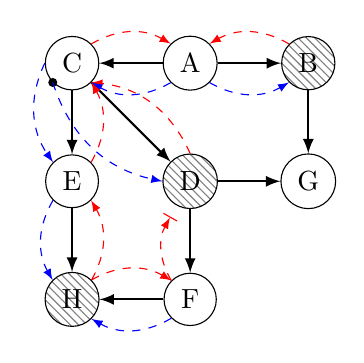
\begin{tikzpicture}[baseline=(current bounding box.center)]
                        % cbr = child below right, pbl = parent below left (snippets)
                        \tikzset{>=latex}
                        \tikzstyle{every node}=[circle, draw=black, node distance=1.5cm]
                        \tikzstyle{every edge}=[black, ->, thick, draw]
                        \node (A) at (0, 0) {A};
                        \node (C) [left of = A] {C};
                        \node[circle, fill=black, inner sep=1pt] at (C.south west) {};
                        \draw (A) edge (C);
                        \node[pattern=north west lines, pattern color=gray] (B) [right of = A] {B};
                        \draw (A) edge (B);
                        \node[pattern=north west lines, pattern color=gray] (D) [below of = A] {D};
                        \draw (C) edge (D);
                        \node (G) [below of = B] {G};
                        \draw (B) edge (G);
                        \draw (D) edge (G);
                        \node (E) [below of = C] {E};
                        \draw (C) edge (E);
                        \node[pattern=north west lines, pattern color=gray] (H) [below of = E] {H};
                        \draw (E) edge (H);
                        \node (F) [below of = D] {F};
                        \draw (D) edge (F);
                        \draw (F) edge (H);
                        
                      \draw[->, blue, dashed, bend right] (C.south west) to 
                                (D.west);

                        \draw[->, red, dashed, bend right] (D.north) to 
                                (C.south east);


                        \draw[->, red, dashed, bend left] (C.north east) to 
                                (A.north west);

                        \draw[->, blue, dashed, bend right] (A.south east) to 
                                (B.south west);

                        \draw[->, red, dashed, bend right] (B.north west) to 
                                (A.north east);


                        \draw[->, blue, dashed, bend left] (A.south west) to 
                                (C.south east);

                        \draw[->, blue, dashed, bend right] (C.west) to 
                                (E.north west);

                        \draw[->, blue, dashed, bend right] (E.south west) to 
                                (H.north west);

                        \draw[->, red, dashed, bend right] (H.north east) to 
                                (E.south east);

                        \draw[->, red, dashed, bend right] (E.north east) to 
                                (C.south east);

                        \draw[->, red, dashed, bend left] (H.north east) to 
                                (F.north west);
                        
                        \draw[->|, red, dashed, bend left] (F.north west) to 
                                ([yshift=-0.2cm]D.south west);

                        \draw[->, blue, dashed, bend left] (F.south west) to 
                                (H.south east);
                        
                \end{tikzpicture}
                                  & $C \indep G \mid B, D, H$ & True \\
                                  \cmidrule{2-3}

                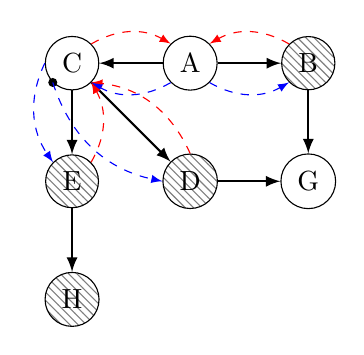
\begin{tikzpicture}[baseline=(current bounding box.center)]
                        % cbr = child below right, pbl = parent below left (snippets)
                        \tikzset{>=latex}
                        \tikzstyle{every node}=[circle, draw=black, node distance=1.5cm]
                        \tikzstyle{every edge}=[black, ->, thick, draw]
                        \node (A) at (0, 0) {A};
                        \node (C) [left of = A] {C};
                        \node[circle, fill=black, inner sep=1pt] at (C.south west) {};
                        \draw (A) edge (C);
                        \node[pattern=north west lines, pattern color=gray] (B) [right of = A] {B};
                        \draw (A) edge (B);
                        \node[pattern=north west lines, pattern color=gray] (D) [below of = A] {D};
                        \draw (C) edge (D);
                        \node (G) [below of = B] {G};
                        \draw (B) edge (G);
                        \draw (D) edge (G);
                        \node[pattern=north west lines, pattern color=gray] (E) [below of = C] {E};
                        \draw (C) edge (E);
                        \node[pattern=north west lines, pattern color=gray] (H) [below of = E] {H};
                        \draw (E) edge (H);
                      \draw[->, blue, dashed, bend right] (C.south west) to 
                                (D.west);

                        \draw[->, red, dashed, bend right] (D.north) to 
                                (C.south east);


                        \draw[->, red, dashed, bend left] (C.north east) to 
                                (A.north west);

                        \draw[->, blue, dashed, bend right] (A.south east) to 
                                (B.south west);

                        \draw[->, red, dashed, bend right] (B.north west) to 
                                (A.north east);


                        \draw[->, blue, dashed, bend left] (A.south west) to 
                                (C.south east);

                        \draw[->, blue, dashed, bend right] (C.west) to 
                                (E.north west);


                        \draw[->, red, dashed, bend right] (E.north east) to 
                                (C.south east);

                                               
                \end{tikzpicture}
                                  & $C \indep G \mid B, D, H, E$ & True \\
                                  \hline
                
                
                
        \end{tabular}
        \caption{Conditional independence statements and active trail 
        (blue dashed paths) shown in the relevant path column for questions (a) to 
        (i).}
        \label{tab:CondIndep1}
\end{table}
\pagebreak 

\begin{table}[H]
        \centering
        \begin{tabular}{ccc}
                Relevant sub-graph &  Conditional independence & True/False \\
                \hline
                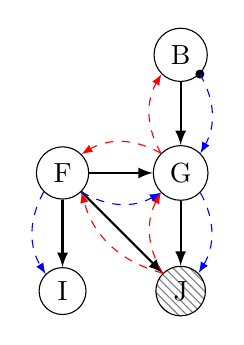
\begin{tikzpicture}[baseline=(current bounding box.center)]
                        % cbr = child below right, pbl = parent below left (snippets)
                        \tikzset{>=latex}
                        \tikzstyle{every node}=[circle, draw=black, node distance=1.5cm]
                        \tikzstyle{every edge}=[black, ->, thick, draw]
                        \node (B) at (0, 0) {B};
                        \node (G) [below of = B] {G};
                        \draw (B) edge (G);
                        \node[pattern=north west lines, pattern color=gray] (J) [below of = G] {J};
                        \draw (G) edge (J);
                        \node (F) [left of = G] {F};
                        \draw (F) edge (G);
                        \node (I) [below of = F] {I};
                        \draw (F) edge (I);
                        \draw (F) edge (J);
                        \node[circle, fill=black, inner sep=1pt] at (B.south east) {};


                        \draw[->, blue, dashed, bend left] (B.south east) to 
                                (G.north east);
                        
                        \draw[->, blue, dashed, bend left] (G.south east) to 
                                (J.north east);

                        \draw[->, red, dashed, bend left] (J.north west) to 
                                (G.south west);

                        \draw[->, red, dashed, bend left] (J.north west) to 
                                (F.south east);


                        \draw[->, red, dashed, bend right] (G.north west) to 
                                (F.north east);


                        \draw[->, red , dashed, bend left] (G.north west) to 
                                (B.south west);

                        
                        \draw[->, blue, dashed, bend right] (F.south west) to 
                                (I.north west);

                        \draw[->, blue, dashed, bend right] (F.south east) to 
                                (G.south west);
                \end{tikzpicture}
                                   & $B \indep I \mid J$ & False \\
                                   \hline
                
        \end{tabular}
        \caption{Conditional independence statement of question (j). In the relevant 
        sub-graph we omitted the node $D$ because we wanted to show the shortest active 
                trail.}
        \label{tab:CondIndep2}
\end{table}



\section{Positive interaction in V-structure}
We let $X,Y,Z$ be binary variables ($\in \{0, 1\} $) with a joint distribution 
parametrized according to the V-structure shown in figure \ref{fig:Vstrct}.
\begin{figure}[H]
        \centering
        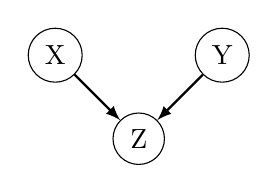
\begin{tikzpicture}
                % cbr = child below right, pbl = parent below left (snippets)
                \tikzstyle{every node}=[circle, draw=black, node distance=1.5cm]
                \tikzstyle{every edge}=[black, ->, thick, draw]
                \node (Z) at (0, 0) {Z};
                \node (Y) [above right of = Z] {Y};
                \draw (Y) edge (Z);
                \node (X) [above left of = Z] {X};
                \draw (X) edge (Z);
                
        \end{tikzpicture}
        
        \caption{V-structure between the binary variables $X, Y$ and $Z$.}
        \label{fig:Vstrct}
\end{figure}

We define the following constant
\begin{align*}
        \alpha &\equiv P(X = 1) \\ 
        \beta &\equiv P(X = 1 \mid Z = 1) \\
        \gamma &\equiv P(X = 1 \mid Z = 1 , Y = 1)
\end{align*}
In term of the marginal $P(X, Y)$ and the conditional $P(Z \mid X, Y)$,
we can rewrite theses constants as follows
\begin{align*}
        \alpha &= \sum_y p(x = 1, y) \\[2ex]
        \beta &= \frac{\displaystyle \sum_y P(X = 1, y) P(Z=1 \mid X=1, y)}{ 
        \displaystyle \sum_x \sum_y P(x, y) P(Z = 1 \mid x, y)} \\[2ex]
                \gamma &=\frac{P(X = 1, Y = 1) P(Z = 1 \mid X = 1, Y = 1)}{
                        \displaystyle
                \sum_x P(x, Y = 1) P(Z = 1 \mid x, Y = 1)} 
\end{align*}
\subsection{Inequalities}
The most general case for $p \in \mathcal{L}(G)$ we can consider where all variable 
are binary random variable is the following 
\begin{align*}
        X & \sim \text{Bernoulli}(p) \\
        Y &\sim \text{Bernoulli}(q) \\[4ex]
        Z \mid X, Y &\sim \left\{ 
                \begin{array}{cc}
                \text{Bernoulli}(\pi_{11}),& \text{if } X = 1 \text{ and } Y = 1 \\
                \text{Bernoulli}(\pi_{10}),& \text{if } X = 1 \text{ and } Y = 0 \\
                \text{Bernoulli}(\pi_{01}),& \text{if } X = 0 \text{ and } Y = 1 \\
                \text{Bernoulli}(\pi_{00}),& \text{if } X = 0 \text{ and } Y = 0 \\
        \end{array}
        \right.
\end{align*}
To simplify the expressions for the constant, we will work with coin flip for $X$ and 
$Y$. Therefore,
\begin{align}
        \label{eq:alpha}
        \alpha &= pq + p(1 - q) = 0.5 \s\s\s \{\text{Since } X \indep Y \mid 
        \emptyset\}\\[3ex]
        \nonumber
        \beta &= \frac{pq\pi_{11} + p(1 - q) \pi_{10}}{pq\pi_{11} + p(1 - q) \pi_{10} + 
        (1 - p)q \pi_{01} + (1 - p)(1 - q)\pi_{00}}  \\[1ex]
        \label{eq:beta}
        &= \frac{\pi_{11} + \pi_{10}}{\pi_{11} + \pi_{10} + \pi_{01} + \pi_{00}} \\[3ex]
        \label{eq:gamma}
        \gamma &=  \frac{pq \pi_{11}}{pq \pi_{11} + (1 - p)q \pi_{01}} = 
        \frac{\pi_{11}}{\pi_{11} + \pi_{01}}
\end{align}



\subsubsection{$\gamma < \alpha$}
Here, we notice that $\pi_{11}$ and $\pi_{01}$ have a big impact on the relative 
importance of $\gamma$ when compared. We can see that 
\begin{align*}
        \pi_{11} \gg \pi_{01} \leq 1 \implies  \gamma \rightarrow 1 \\
        \pi_{01} \gg \pi_{11} \leq 1 \implies  \gamma \rightarrow 0
\end{align*}
Setting every other parameter to $0.5$, $\pi_{11} = 0.01$ and $\pi_{01} = 0.9$, we get 
the following example for which $\gamma < \alpha$
\renewcommand{\arraystretch}{1}
\begin{table}[H]
\begin{minipage}{.45\textwidth}
        \centering
        
        \begin{tabular}{|c|c|c|}
                \hline
                X & Y & P(X, Y) \\  \hline
                1 & 1 & 0.25 \\\hline 
                1 & 0 & 0.25 \\\hline 
                0 & 1 & 0.25 \\\hline 
                0 & 0 & 0.25 \\\hline
        \end{tabular}
        \caption{Joint distribution of 2 coin flip.}
\end{minipage}
\begin{minipage}{.45\textwidth}
        \centering
        \begin{tabular}{|c|c|c|}
                \hline
                X & Y & $P(Z = 1 \mid X, Y)$ \\\hline
                1 & 1 & 0.01 \\\hline
                1 & 0 & 0.5 \\\hline
                0 & 1 & 0.9 \\\hline
                0 & 0 & 0.5 \\\hline
        \end{tabular}
        \caption{Conditional on $Z = 1$ with $\gamma \ll 1$.}
\end{minipage}
        \label{tab:Joint1}
\end{table}

\begin{table}[H]
        \centering
        \begin{tabular}{|c|c|c|}
                \hline 
                $\alpha$ & $\beta$ & $\gamma$ \\ \hline 
                0.5 & 0.28 & 0.01 \\\hline
        \end{tabular}
        \caption{Results}
        \label{tab:Res1}
\end{table}



\subsubsection{$\alpha < \gamma < \beta$}
$\gamma > \alpha$ can be obtained by setting $\pi_{11} \gg \pi_{01}$. To get 
the RHS of the inequality, we must set $\pi_{00}\ll 1$.
The following table works as intended:
\begin{table}[H]
\begin{minipage}{.45\textwidth}
        \centering
        
        \begin{tabular}{|c|c|c|}
                \hline
                X & Y & P(X, Y) \\  \hline
                1 & 1 & 0.25 \\\hline 
                1 & 0 & 0.25 \\\hline 
                0 & 1 & 0.25 \\\hline 
                0 & 0 & 0.25 \\\hline
        \end{tabular}
        \caption{Joint distribution of 2 coin flip.}
\end{minipage}
\begin{minipage}{.45\textwidth}
        \centering
        \begin{tabular}{|c|c|c|}
                \hline
                X & Y & $P(Z = 1 \mid X, Y)$ \\\hline
                1 & 1 & 0.9 \\\hline
                1 & 0 & 0.5 \\\hline
                0 & 1 & 0.5 \\\hline
                0 & 0 & 0.001 \\\hline
        \end{tabular}
        \caption{Conditional on $Z = 1$ with $\gamma \ll 1$.}
\end{minipage}
        \label{tab:Joint2}
\end{table}

\begin{table}[H]
        \centering
        \begin{tabular}{|c|c|c|}
                \hline 
                $\alpha$ & $\beta$ & $\gamma$ \\ \hline 
                0.5 & 0.74 & 0.64 \\\hline
        \end{tabular}
        \caption{Results}
        \label{tab:Res2}
\end{table}

\subsubsection{$\beta < \alpha < \gamma$}
Here, starting from equilibrium (all parameter equal), we can shift $\beta$ to 
be smaller than the other by increasing $\pi_{00}$. Then we can increase 
$\gamma$ slightly by increasing slightly $\pi_{11}$. Too harsh an 
increase will upset the lower inequality.

\begin{table}[H]
\begin{minipage}{.45\textwidth}
        \centering
        
        \begin{tabular}{|c|c|c|}
                \hline
                X & Y & P(X, Y) \\  \hline
                1 & 1 & 0.25 \\\hline 
                1 & 0 & 0.25 \\\hline 
                0 & 1 & 0.25 \\\hline 
                0 & 0 & 0.25 \\\hline
        \end{tabular}
        \caption{Joint distribution of 2 coin flip.}
\end{minipage}
\begin{minipage}{.45\textwidth}
        \centering
        \begin{tabular}{|c|c|c|}
                \hline
                X & Y & $P(Z = 1 \mid X, Y)$ \\\hline
                1 & 1 & 0.6 \\\hline
                1 & 0 & 0.5 \\\hline
                0 & 1 & 0.5 \\\hline
                0 & 0 & 0.9 \\\hline
        \end{tabular}
        \caption{Conditional on $Z = 1$ with $\gamma \ll 1$.}
\end{minipage}
        \label{tab:Joint3}
\end{table}

\begin{table}[H]
        \centering
        \begin{tabular}{|c|c|c|}
                \hline 
                $\alpha$ & $\beta$ & $\gamma$ \\ \hline 
                0.5 & 0.44 & 0.54 \\\hline
        \end{tabular}
        \caption{Results}
        \label{tab:Res3}
\end{table}


\subsection{}

\subsubsection{$\gamma < \alpha$}
In order for this inequality to hold, then the effect $Z = 1$ must contain information 
about a correlation between the causes $Y = 1$ and the possible values of $X$.
This information is encoded 
through the parameters $\pi_{11}$ and $\pi_{01}$. By lowering $\pi_{01}$, we 
naturally lower the possibility that $X = 0$ given $Z = Y = 1$. Conversely 
for $\pi_{11}$. Therefore, the condition $\pi_{01} \ll \pi_{11} \leq 1$, 
all other parameters being equal, means that the observation of the effect $Z = 1$ 
and the cause $Y = 1$ update strongly our belief about the probability of observing $X = 1$. 
Initially, we had no particular opinion $\alpha = 0.5$. After observation, we are now 
almost convinced that the second cause was $X = 1$.


\subsubsection{$\alpha < \gamma < \beta$}
Here, we reversed the previous inequality first so that the observation of $Y = 1$ 
and the observation of the effect $Z = 1$ will increase the probability of observing 
$X = 1$. The RHS can function independently of the first one since $\pi_{00}$ 
do not affect $\gamma$. Indeed, $Y = 1$ is observed for $\gamma$ therefore
the probability 
of observing $Y = 0$ do not impact $\gamma$. \par
For the $\beta$ probability, we are working with less information about the cause 
of $Z = 1$ (we do not know $Y$). Therefore, to have higher confidence of observing 
$X = 1$ without knowing the $Y$ cause means we must have a strong belief that 
observing the effect $Z = 1$ means the cause $X = 0$ is unlikely. 
This is encoded in $\pi_{00}$
and $\pi_{01}$ (but we do not touch this one in order to keep $\gamma$ intact).
This is why setting $\pi_{00}$ to a low value yielded the inequality we seeked.

\subsubsection{$\beta < \alpha < \gamma$}
Here, we want to lower our confidence that observing $Z = 1$ was caused by 
$X = 1$. To do that, we bring $\pi_{00}$ to a very probable value. This 
update our belief that an effect $Z = 1$ is most likely caused by $X = 0$ when 
$Y = 0$. We do not increase $\pi_{01}$ because we do not want to lower our 
confidence that observing $Z = 1$ and $Y = 1$ is related to an event with 
$X = 1$ ($\gamma$). This is why we increase only slightly $\pi_{11}$ in order to 
increase $\gamma$ without upsetting too much $\beta$. 

In other words, observing the effect $Y = 1$ will increase slightly our confidence 
that the second cause for $Z = 1$ was $X = 1$ as opposed to no belief at all 
($\alpha$), updating our initial belief that the 
most probable cause was $X = 0$.


\section{Equivalence of DGM with UGM}
We consider a directed tree graphical model $G = (V, E)$. By definition, each nodes has at most 
one parent 
\[
        |\pi_i| \leq 1\s \forall \s i \in V 
\]
A distribution $p$ is part of the family of distribution $\mathcal{L}(G)$
associated with the graph $G$ if it has legal factors $\{f_i\}$ associated with
the conditional 
independences of $G$
\[
        \mathcal{L}(G) = \left\{ \text{p is a distribution over }\, X_V
        \,\middle\vert\, 
        p(X_V) = \prod_{i} f_i(x_i \mid x_{\pi_i})
        \right\}
\]

The moralized graph $\bar{G}$, is the UGM associated with $G$. It has cliques 
of size at most 2 since no edges will be added to the tree in the moralization 
procedure. 
\[
        \max |C| \leq |\pi_i| + 1 \s \forall i \in V\s \text{and } 
        \forall \s C \s \in \mathscr{C}_{\max}
\]
where $\mathscr{C}_{\max}$ is the set of maximal cliques in $\bar{G}$.
This is to say that all cliques will have two nodes. The 
factorization of a UGM is done over all maximal cliques:
\[
        \mathcal{L}(\bar{G}) = \left\{   \text{p is a distribution over }\, X_V
        \,\middle\vert\, 
        p(X_V) = \frac{1}{Z} \prod_{C \in \mathscr{C}_{\max}} \psi_C(x_C) 
 \right\}
\]
The notion of factor here can be loosely defined as a function of a subset 
of nodes of the graphs. Using the definition of $\mathcal{L}(G)$ and 
$\mathcal{\bar{G}}$, we define the equality of these sets if we can find 
a bijective map between the factors of $p_{G_n}$ and $p_{\bar{G}_n}$ for 
any $n \geq 1$.


\begin{proof}
        Let $G_n = (V, E)$ be a directed tree of size $n = |V|$, the number of nodes 
        in that tree. 
        We first set $n = 1$. In this case, 
        \[
                p_{G_1}(X_V) = f_1(x_1)
        \]
        and
        \[
                p_{\bar{G}_1}(X_V) \propto \psi_1(x_i)
        \]
        The two distributions have the same factorization and belongs to the same family.
        Therefore, 
        \[
                \mathcal{L}(G_1) = \mathcal{L}(\bar{G}_1)
        \]

        For $n = 2$, 
        \[
                p_{G_2}(X_V) = f_1(x_1)f_2(x_2 \mid x_1)
        \]
        and
        \[
                p_{\bar{G}_2}(X_V) \propto \psi_1(x_1,  x_2) 
        \]
        since there is only one clique of the maximal size in that set. 
        We make the following map between the two parametrization:
        \[
                \psi_1(x_1, x_2)
                \overset{1:1}{\longleftrightarrow}
                \underbrace{f_1(x_1)f_2(x_2 \mid x_1)}_
                {\displaystyle f_1(x_1, x_2)}
        \]
        $f_1(x_1)f_2(x_2 \mid x_1)$ 
        is a single factor over the set of variables $\{x_2, x_2\}$. 

        This is trivially a bijective map (one-to one mapping) 
        between the two sets of factors. The 
        set of distribution that can be represented by $G_2$ is equal to the 
        set of distribution represented by $\bar{G}_2$
        \[
                \mathcal{L}(G_2) = \mathcal{L}(\bar{G}_2)
        \]

        Now, we assume that $\mathcal{L}(G_n) = \mathcal{L}(\bar{G}_n)$ is true. 
        This is to say that there exist a bijective map between 
        $\{f_i\}_{i=1,\dots,n}$ and $\{\psi_i\}_{i=1,\dots,n}$:
        \begin{enumerate}
                \item Each element of $\{\psi_i\}$ 
                        is paired with at least one element of $\{f_i\}$;
                \item No element of $\{\psi_i\}$ is paired with more than 
                        one element of $\{f_i\}$;
                \item Each element of $\{f_i\}$ is paired with at least 
                        one element of $\{psi_i\}$;
                \item No element of $\{f_i\}$ is paired with more than 
                        one element of $\{\psi_i\}$.
                
        \end{enumerate}

        For $n + 1$, we have
        \[
                p_{G_{n + 1}}(X_V) = \prod_{i = 1}^{n+1} f_i(x_i \mid p_{\pi_i})
        \]
        Since $\pi_{n +1} = n$, 
        \[
                p_{G_{n + 1}}(X_V) = f_{n + 1}(x_{n + 1} \mid x_{n})\prod_{i = 1}^{n} 
                f_i(x_i \mid x_{\pi_i}) = f_{n + 1}(x_{n + 1} \mid x_n) p_{G_n}(X_V)
        \]
        On the other hand
        \[
                p_{\bar{G}_{n + 1}}(X_V) = \frac{1}{Z} \prod_{C \in \mathscr{C}_{\max}} 
                \psi_C (x_C)
        \]
        Since all cliques are of length 2, we can factor out the clique 
        \[
                C_{n + 1} = \{x_{n + 1}, x_n\} 
        \]
        \[
                p_{\bar{G}_{n + 1}}(X_V) = \frac{1}{Z} \psi_{C_{n + 1}}(x_{n + 1}, x_n) 
                \prod_{C \in \mathscr{C}_{\max} \setminus C_{n + 1}} \psi_C(x_C)
        \]
        Ignoring the normalization constant, this is 
        \[
                p_{\bar{G}_{n + 1}}(X_V) 
                \propto \psi_{C_{n + 1}}(x_{n + 1}, x_n) p_{\bar{G}_n}(X_V)
        \]
        Since we know there exist a bijective map of the factors for the graph of 
        $n$ nodes, then we have found that $G_{n + 1}$ also have a bijective 
        map between its factors because the additional factor of $G_{n + 1}$ 
        and $\bar{G}_{n + 1}$ are mapped exclusively between themselves:
        \[
                \psi_{C_{n + 1}}(x_{n + 1}, x_n) 
                \overset{1:1}{\longleftrightarrow} f_{n + 1}(x_{n + 1} \mid x_n)
        \]
        Therefore
        \[
                \mathcal{L}(G_{n + 1}) = \mathcal{L}(\bar{G}_{n + 1})
        \]
        The statement 
        \[
                \mathcal{L}(G_n) = \mathcal{L}(\bar{G}_{n+1}),\s \forall \s n
                \in \mathbb{N}^+
        \]
        is proved by induction.

\end{proof}



\section{Hammersley-Clifford Counter-Example}
\begin{namedtheorem}[Hammersley-Clifford]
Suppose $\mathcal{UI}$ is the set of positive distributions that satisfy the global Markov 
property of the Markov network $G = (V, E)$. 
\[
        p(X_V) \models (X \indep Y \mid Z),\s\s \text{s.t.}\s\s \text{sep}_G(X ;Y \mid Z)
\]
for the disjoint sets $X$, $Y$ and $Z$ in $V$.
Then, suppose that  
 $\mathcal{UF}$ is the set of Gibbs distributions that can be expressed as a factorization 
of the form 
\[
        p(X_V) = \frac{1}{Z} \prod_{C \in \mathscr{C}_{\max}} \psi_C(x_C)
\]
Then
\[
        \mathcal{UI} = \mathcal{UF}
\]
\end{namedtheorem}

We can show that a probability distribution that is not strictly positive 
will not factorize according to the set of distributions $\mathcal{UF}$, 
even if it respect 
the global Markov property of the graph $G$.

We consider the following graph
\begin{figure}[H]
        \centering
        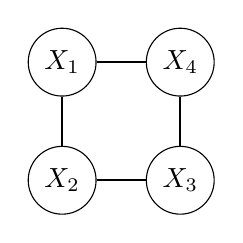
\begin{tikzpicture}
                % cbr = child below right, pbl = parent below left (snippets)
                %\tikzset{>=latex}
                \tikzstyle{every node}=[circle, draw=black, node distance=1.5cm]
                \tikzstyle{every edge}=[black, -, thick, draw]
                \node (X1) at (0, 0) {$X_1$};
                \node (X2) [below of = X1] {$X_2$};
                \draw (X1) edge (X2);
                \node (X3) [right of = X2] {$X_3$};
                \draw (X2) edge (X3);
                \node (X4) [above of = X3] {$X_4$};
                \draw (X4) edge (X3);
                \draw (X4) edge (X1); 
        \end{tikzpicture}
        
        \caption{A Markov Network of binary variables.}
        \label{fig:HCMarkovNetwork}
\end{figure}
And consider the following probability distribution
\[
        P(X_V) = \left\{ 
                \begin{matrix}
                        \dfrac{1}{8},& \text{if }\, X_V \in \Xi \\[3ex]
                        0,& \text{otherwise}

                        
                \end{matrix}
        \right.
\]
Where we have created the set 
\[
        \Xi = \left\{
                \begin{matrix}
                        (0,\ 0,\ 0,\ 0),\ (1,\ 0,\ 0,\ 0),\ (1,\ 1,\ 0,\ 0), 
                        (1,\ 1,\ 1,\ 0),\ \\[2ex] (0,\ 0,\ 0,\ 1),\ 
                        (0,\ 0,\ 1,\ 1),\ (0,\ 1,\ 1,\ 1),\ 
                        (1,\ 1,\ 1,\ 1)
                \end{matrix}
        \right\}
\]
We do not show that $P$ satisfy the global Markov property, and take it for 
granted since it can be proved easily by showing that conditioning on 
any set $Z$ that separates $X$ and $Y$ will make $X$ and $Y$ deterministically 
determined on $Z$, making $X$ and $Y$ independent.

Here, we prove that $P(X_V) \not\in \mathcal{UF}$:
\begin{proof}
        Suppose that $P(X_V) \in \mathcal{UF}$. Then, it can be factorized 
        over the set of maximal cliques of $G$:
        \[
                P(X_V) = \frac{1}{Z} \phi_1(X_1, X_2) \phi_2(X_1, X_4) 
                \phi_3(X_2, X_3) \phi_4(X_3, X_4)
        \]
        We consider the case $p(0, 1, 1, 0) = 0$. To have a null probability, 
        we could have $Z = \infty $, but this would not be consistent with 
        the distribution $P(X_V)$ since $Z$ is common to all $X_V$.

        Another solution is to set one of the factor $\phi_i$ to $0$. 
        Suppose we set 
        \[
                \phi_1(0, 1) = 0
        \]
        Then, 
        \[
                p(0, 1, 1, 1) = \frac{1}{Z}\phi_1(0, 1)\phi_2(0, 1) 
                \phi_3(1, 1) \phi_4(1, 1) = 0
        \]
        But, the distribution we started with assumes $P(0, 1, 1, 1) = \frac{1}{8}$ 
        so we must have $\phi_1(0, 1) \not= 0$. 
        Going over all other possibilities, we find that no factor can be 
        set to 0.
        \begin{align*}
                p(0, 0, 0, 0) = \frac{1}{8} &\implies \phi_2(0, 0) \not= 0\\
                p(0, 1, 1, 1) = \frac{1}{8} &\implies \phi_3(1, 1) \not= 0 \\
                p(1, 1, 1, 0) = \frac{1}{8} &\implies \phi_4(1, 0) \not= 0
        \end{align*}
        We find that there is no way to have $p(0, 1, 1, 0) = 0$ given the 
        factorisation in $\mathcal{UF}$.
        This is a contradiction, and we conclude that $P(X_V) \not\in \mathcal{UF}$.

\end{proof}


\section{Bizarre Conditional Independence Properties}
We let $(X, Y, Z)$ be a random vector with a finite sample size. We consider 
the following statement
\begin{equation}\label{eq:Statement}
        \text{If } X \indep Y \mid Z \s \text{and } X \indep Y \mid \emptyset
        \implies  (X \indep Z \mid \emptyset \s \text{or } Y \indep Z \mid \emptyset )
\end{equation} 
We suppose the premiss to be true. This put a limitations on the family of distributions 
that are allowed. We show in the figure below the allowed graphical representations 
of those distributions.

\begin{figure}[H]
        \centering
        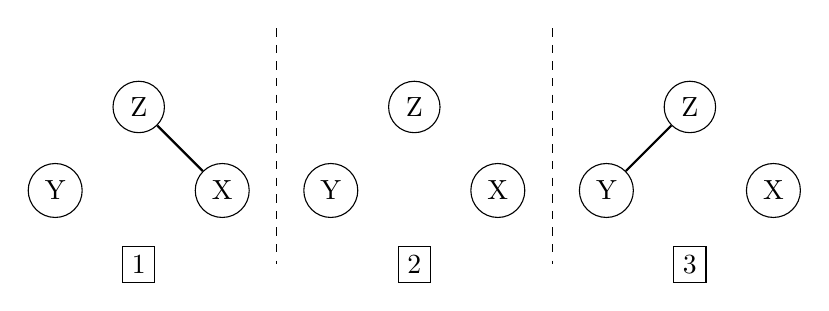
\begin{tikzpicture}
                % cbr = child below right, pbl = parent below left (snippets)
                %\tikzset{>=latex}
                \tikzstyle{every node}=[circle, draw=black, node distance=1.5cm]
                \tikzstyle{every edge}=[black,  thick, draw]
                \node (Z) at (0, 0) {Z};
                \node (X) [below right of = Z] {X};
                %\draw (Z) edge (X);
                \node (Y) [below left of = Z] {Y};
                %\draw (Z) edge (Y);

                \node[rectangle] at (0, -2) {2};

                \draw[dashed] (1.75, 1) -- (1.75, -2);
                \node (Z) at (3.5, 0) {Z};
                \node (X) [below right of = Z] {X};
                %\draw (Z) edge (X);
                \node (Y) [below left of = Z] {Y};
                \draw (Z) edge (Y);


                \node[rectangle] at (-3.5, -2) {1};

                \draw[dashed] (-1.75, 1) -- (-1.75, -2);
                \node (Z) at (-3.5, 0) {Z};
                \node (X) [below right of = Z] {X};
                \draw (Z) edge (X);
                \node (Y) [below left of = Z] {Y};
                %\draw (Z) edge (Y);
                
                \node[rectangle] at (3.5, -2) {3};
                
        \end{tikzpicture}
        
        \caption{Only 3 allowed graph configuration.}
        \label{fig:}
\end{figure}
Those are the only possible configurations because a third link 
between the 3 random variables will make one of the two premiss false. 
For example, if we consider $Z$ to be a common cause to $X$ and $Y$, 
then $X \indep Y \mid Z$ is true but $X$ and $Y$ are not marginally 
independent. If we would consider a v-structure, then the conditional 
independence statement would be false. The same hold true for a UGM.

To prove the implication, we go through all possible graphs. The graph labeled 2
implies that all variable are both marginally independent and 
conditionally independent since there is no edges. Therefore, 
\[
        2 \implies X \indep Z \s \text{and } Y \indep Z 
\]
The graphs 1 and 3 have one edge, for which one of the independence statements 
will fail
\[
        1 \implies Y \indep Z ,\s\s 3 \implies Z \indep X
\]
Doing a truth values table, we find that of all the possible cases, the statement 
\[
         X \indep Y \mid Z \s \text{and } X \indep Y \mid \emptyset
        \implies  (X \indep Z \mid \emptyset \s \text{or } Y \indep Z \mid \emptyset )
\]
always holds. This is true for any positively defined distribution with finite support 
and infinite support. $\qed$



\section{EM and Gaussian Mixture}
\subsubsection{Primer}

The Gaussian Mixture Model is a graphical model with a random categorical latent 
variable $\mathbf{z}_i$ and deterministic parameters 
$$\theta = (\pi_{1,\dots,K}, (\mu_i)_{i = 1}^K, (\Sigma_i)_{i = 1}^K)^T.$$
\begin{figure}[H]
        \centering
        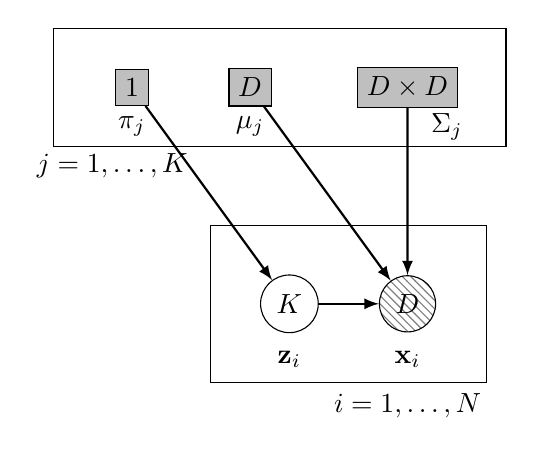
\begin{tikzpicture}
                \tikzstyle{every node}=[node distance=1.5cm]
                %\tikzstyle{every edge}=[black, ->, thick, draw]
                \node[circle, draw] (zi) at (0,0) {$K$};
                \node[circle, draw, pattern=north west lines, pattern color=gray] (x) 
                        [right of = zi] {$D$};
                \node at (0, -0.7) {$\mathbf{z}_i$};
                \node at (1.5, -0.7) {$\mathbf{x}_i$};
                \draw[->, thick, draw] (zi) edge (x);
                \draw (-1, 1) rectangle (2.5, -1);
                \node at (1.5, -1.3) {$i = 1,\dots, N$};

                \draw (-3, 3.5) rectangle (2.75, 2);
                \node[rectangle, draw, fill=gray!50] (pi) at (-2, 2.75) {1};
                \draw[->, thick] (pi) edge (zi);
                \node at (-2, 2.25) {$\pi_j$};

                \node[rectangle, draw, fill=gray!50] (mu) [right of = pi] {$D$};
                \node at (-0.5, 2.25) {$\mu_j$};
                \draw[->, thick] (mu) edge (x);

                \node[rectangle, draw, fill=gray!50, node distance=2cm]
                        (sigma) [right of = mu] {$D \times D$};
                \node at (2, 2.25) {$\Sigma_j$};
                \draw[->, thick] (sigma) edge (x);

                \node at (-2.25, 1.75) {$j = 1, \dots, K$};
                
                
                
        \end{tikzpicture}
        \caption{Gaussian Mixture Model with plate notation. The label inside the circles 
        are references to the vector dimension. $\mathbf{z}_i$ is a $K$-vector, etc.}
        \label{fig:GMM}
\end{figure}



There is a  latent variable $\mathbf{z}_i$ for each observations ($i=1,\dots, N$) and latent variables $\mu_j$ and $\Sigma_j$ for each cluster $j = 1,\dots,K$. The $z_{i}$ are distributed with a $K$-Categorical distribution. The Multinoulli is a natural choice.
$$
  \mathbf{z}_i \sim \text{Multinoulli}(\pi_{1,\dots,K})
$$
We then assume the conditional over an observation $\mathbf{x}_i$ assigned to the cluster $j$ ($z_{i, j} = 1$) to follow a multivariate normal distribution
$$
\mathbf{x}_i \mid z_{i, j} = 1 \sim \mathcal{N}(\mu_j, \Sigma_j)
$$
where $\mathbf{x}$ and $\mu_j$ are $D$-vectors, and the covariance 
matrix is a positive semi-definite, symmetric $D \times D$ matrix. We define 
the complete log-likelihood (a lower bound on the log-likelihood with missing 
information):
$$
\mathcal{L}_C = \log p(\mathbf{x}, \mathbf{z} \mid  \theta) = \sum_{i = 1}^N \sum_{j = 1}^K
    z_{i, j} \log \mathcal{N}(\mathbf{x}_i \mid \mu_j , \Sigma_j) 
    + z_{i, j} \log \pi_j
$$

We take the expectation of that likelihood 

$$
 \mathbb{E}_q\left[\log p(\mathbf{x}, \mathbf{z} \mid  \theta) \right] 
 =  \sum_{i = 1}^N \sum_{j = 1}^K
    \mathbb{E}_q[z_{i, j}] (\log \mathcal{N}(\mathbf{x}_i \mid \mu_j , \Sigma_j) 
    +  \log \pi_j)
$$
The expectation is taken with respect to the marginal distribution 
of the cluster assignement variable $z_i$:
$$
 q^{(t + 1)}(\mathbf{z}) = p(\mathbf{z} \mid \mathbf{x}_i , \theta^{(t)})
$$
For a single observation, this is 
$$
  q^{(t + 1)}(\mathbf{z}_i) = p(\mathbf{z}_i \mid \mathbf{x}_i , \theta^{(t)})
$$
Using Bayes theorem, 
$$
  q^{(t + 1)}(\mathbf{z}_i) = \frac{p(\mathbf{x}_i \mid \mathbf{z}_i,  \theta^{(t)}) p(\mathbf{z}_i \mid \pi^{(t)})}{p(\mathbf{x}_i \mid \theta^{(t)})}
$$
We define the weight 
$\Upsilon_{i, j}$ to be the probability 
$\Upsilon_{i, j}^{(t + 1)} = q^{(t + 1)}(z_{i, j} = 1)$.
Using the expressions for the conditional and the prior on the 
latent variable $z_{i, j} = 1$, we can write
$$
\mathbb{E}_{q^{(t + 1)}}(z_{i, j}) = 
        \Upsilon^{(t + 1)}_{i, j} = 
        \frac{
                \pi_j^{(t)} \mathcal{N}(\mathbf{x}_i \mid \mu_j^{(t)}, \Sigma_j^{(t)})
                }{
                \displaystyle \sum_{\ell = 1}^K \pi_\ell^{(t)}
                \mathcal{N}(\mathbf{x}_i \mid \mu_\ell^{(t)}, \Sigma_\ell^{(t)})
} 
$$
At the maximization step, we do the constrained optimization
for the deterministic parameters using the Lagrange multiplier $\lambda$
$$
\theta^{(t + 1)} \overset{\Delta}{=} \underset{\theta}{\text{argmax }} 
\mathbb{E}_{q^{(t +1)}} [\log p(\mathbf{x}, \mathbf{z} \mid \theta)] + \lambda 
\left(1 - \sum_{j = 1}^{K} \pi_j\right)
$$
Writing out all the terms except the constant term, 
\[
        \theta^{(t+1)} =  \underset{\theta}{\text{argmax }} 
        \sum_{i = 1}^{N} \sum_{j = 1}^{K}\Upsilon_{i, j}^{(t + 1)} 
        \left( 
        \frac{1}{2}\log \det \Sigma^{-1}
        - \frac{1}{2} (\mathbf{x}_i - \mu_j)^T \Sigma^{-1}_j (\mathbf{x}_i - \mu_j)
        + \log \pi_j
        \right)
        +
        \lambda\left(1 - \sum_{j = 1}^{K} \pi_j\right)
\]


\subsubsection{M-step for $\pi_j$}
\[
        \partial_{\pi_\ell} \mathcal{L} = \sum_{i=1}^{N} \sum_{j = 1}^{K} 
        \Upsilon_{i, j}^{(t + 1)} \frac{\delta_{j \ell}}{\pi_j} 
        - 
        \lambda
\]
where $\delta_{j\ell}$ is the Kronecker delta coming from the partial derivate.
The MLE solution is found where this derivative is 0:
\[
        \hat{\pi}_\ell = \frac{1}{\hat{\lambda}}\sum_{i = 1}^{N}
        \Upsilon_{i,\ell}^{(t + 1)} 
\]
From the constraint, we have
\[
        \frac{1}{\hat{\lambda}}\sum_{j = 1}^{K}\sum_{i = 1}^{N} 
        \Upsilon_{i, j}^{(t+1)} = 1
\]
But
\[
        \sum_{j = 1}^{K}\Upsilon_{i, j} = 1
\]
Therefore, $\lambda = N$ and the MLE solution is 
\[
        \boxed{\hat{\pi}_\ell = \frac{1}{N}\sum_{i = 1}^{N} \Upsilon_{i, \ell}^{(t+1)}}
\]


\subsubsection{M-step for $\mu_j$}
\[
        \partial_{\mu_\ell} \mathcal{L} = \sum_{i = 1}^{N} \sum_{j = 1}^{K} 
        \Upsilon_{i, j}^{(t+1)}\Sigma^{-1}_j(\mathbf{x}_i - \mu_j) \delta_{j, \ell}
\]
At the stationary point, we can simplify the covariance matrix and we get 
\[
        0 = \sum_{i = 1}^{N} \Upsilon_{i, \ell}^{(t+1)}\mathbf{x}_i 
        - \hat{\mu}_\ell\sum_{i = 1}^{N}\Upsilon_{i, \ell}^{(t+1)}
\]
Therefore, 
\[
      \boxed{  \hat{\mu}_{\ell} = \frac{1}{\displaystyle \sum_i \Upsilon_{i, \ell} 
      ^{(t+1)}} \sum_{i = 1}^{N} \Upsilon_{i, \ell}^{(t + 1)} \mathbf{x}_i}
\]
\subsubsection{M-step for $\Sigma_j$}
We will derive the full form of the update, and give the special result for a 
diagonal covariance matrix at the end. To simplify the derivative, we derive 
with respect to $\Lambda \equiv \Sigma^{-1}$:
\[
        \partial_{\Lambda_\ell} \mathcal{L} = \sum_{i = 1}^{N} \sum_{j = 1}^{K} 
        \Upsilon_{i, j}^{(t+1)}
        \left(\frac{1}{2} \Sigma_j 
                - \frac{1}{2}
        (\mathbf{x}_i - \hat{\mu}_j)(\mathbf{x}_i - \hat{\mu}_j)^{T} \right) \delta_{j \ell} 
\]
At the stationary point, this gives
\[
        \hat{\Sigma}_\ell =
        \frac{1}{\displaystyle\sum_{i = 1}^{N} \Upsilon_{i, \ell}^{(t+1)} } 
        \sum_{i = 1}^{N} \Upsilon_{i, \ell}^{(t + 1)} 
        (\mathbf{x}_i - \hat{\mu}_\ell)(\mathbf{x}_i - \hat{\mu}_\ell)^{T}
\]
Assuming a spherical covariance matrix $\Sigma_j = \sigma^{2}_j\mathbf{1}$, then 
the terms involving the covariance become scalars. The gradient will 
also be a scalar: 
\[
        \partial_{\sigma^{-2}_\ell} \mathcal{L} = 
        \sum_{i = 1}^{N} \sum_{j =1}^{K}
        \Upsilon_{i, j}^{(t + 1)}
        \left(  
                \frac{1}{2}\sigma^{2}_j - \frac{1}{2}(\mathbf{x}_i - \hat{\mu}_j)^{T} 
                (\mathbf{x}_i - \hat{\mu}_j)
\right)\delta_{j \ell}
\]
At the stationary point, we get a similar expression to the previous one, but this 
time scalar:
\[
       \boxed{ \hat{\sigma}^{2}_\ell = \frac{1}{\displaystyle 
        \sum_{i = 1}^{N} \Upsilon_{i, \ell}^{(t+1)}} 
        \sum_{i = 1}^{N} \Upsilon_{i,\ell}^{(t+1)} (\mathbf{x}_i - \hat{\mu}_\ell)^{T} 
(\mathbf{x}_i - \hat{\mu}_\ell)}
\]
%We outline here the EM algorithm for the GMM:

  %1. Initialize $\mu^{(1)}$ with k-means++;
  %2. Initialize $\Sigma_j^{(1)}$ with a large spherical covariance $\sigma^2 \mathbf{1}$, $\sigma^2 \gg 1$;
  %3. Initialize $\pi_j^{(1)}$ with the proportions of each class from k-means++;
  %4. Iterate until convergence ()


\section{Appendix}
\subsection{Bayes Ball algorithm}
Here we focus our attention to the Bayes Ball algorithm for probabilistic node only. In that 
case, conditional independence $X_J \indep X_L \mid X_K$, with $J,K,L \subseteq V$ requires 
the notion of d-separation:
\begin{description}
        \item{\textbf{Active path}} An active path from $J$ to $L$ given $K$ is 
                an undirected path between $\ell \in L$ and $j \in J$ such that every 
                node $i$ with two parents in this chain is observed ($i \in K$) or 
                has a descendant in $K$
        \item{\textbf{D-separation}} $X_j$ is said to be conditionally independent to 
                $X_L$ (or 
                \textit{d-separate} $X_L$) given $X_K$ if there is no active path 
                from $J$ to $L$ given $K$.
\end{description}
With this description, we can devise a simple algorithm that will find all active 
path in the graph in linear time \cite{BB}. We will use the following convention 
\begin{itemize}
        \item $\color{blue} \dashrightarrow $ Dashed blue arrows indicate the ball drop from parent to child;
        \item $\color{red} \dashrightarrow$ Dashed red arrow indicate the ball bounce back to the 
                parent;
        \item Barred arrows mean the node will block the ball (neither bounce it back 
                nor let it pass through). These can be used as an indicator and are not 
                necessary for the algorithm.
\end{itemize}
With this convention, we describe an algorithm that will find all active path 
from a node $\ell \in L$ to a node $j \in J$ given 
$K$ if they exists:

\begin{algorithm}[H]
        \KwResult{active paths in the graph $\color{blue} \dashrightarrow$}
        initialize a schedule with all $j \in J$ as though they were  
        visited by a child\;
        \While{schedule not empty}{ 
                pick a node $j$ and remove it from the schedule\;
                \If{$j \not\in K$ \textbf{and} 
                        $j$ is visited from a child \textbf{and} there is no 
                        $\color{red} \dashrightarrow$ linking $j$ to previous node}{
                        draw $\color{red} \dashrightarrow$ going into $j$\;
                        schedule its parents to be visited\;
                        schedule its children to be visited\;
                }
                \uElseIf{$j$ is visited from a parent \textbf{and} there is no 
                        $\color{blue} \dashrightarrow$ linking $j$ to previous node}{
                        draw $\color{blue} \dasharrow$ going into $j$\;
                        \eIf{$j \in K$}{
                                schedule its parents to be visited\;
                        }{
                        schedule its children to be visited\;
                }
                        
        }
        }

        \caption{Bayes Ball} 
        \label{alg:Bayes}
\end{algorithm}
%With this description of conditional independence, a simple algorithm given only 
%two simple rules:
%\begin{itemize}
        %\item An unobserved node pass the ball through and bounce it back to its 
                %parent;
        %\item An observed node bounce back the ball from the parents, and block the 
                %ball for the children.
%\end{itemize}
%To determine we start from a node in $J$ and search for an active path that leads to $L$ 
%given $K$.



\begin{thebibliography}{9}
        \bibitem{BB}
        Shachter, R. D. (2013). 
        Bayes-Ball: The Rational Pastime (for Determining Irrelevance and Requisite Information in Belief Networks and Influence Diagrams). \url{http://arxiv.org/abs/1301.7412}
        
\end{thebibliography}

\end{document}

